\documentclass{jsarticle}

\usepackage{amsmath}
\usepackage[dvipdfmx]{graphicx,color}
\usepackage[dvipdfmx,colorlinks=true,linkcolor=black,urlcolor=blue]{hyperref}
\usepackage{url}
\usepackage{wrapfig}

\begin{document}

\title{
  \textbf{Bancorプロトコル}
  \protect\linebreak
  \protect\linebreak
  \large
  スマートコントラクトを通じて、トークンの継続的な流動性と非同期的な価格発見を可能にする「スマートトークン」について
}

\author{Eyal Hertzog, Guy Benartzi \& Galia Benartzi}
\date{May 30, 2017}

\maketitle

\begin{center}
  \item[訳者:] \href{https://kentarok.org}{栗林 健太郎}
  \item[原本:] \href{http://www.hyuki.com/girl/}{Draft Version 0.99}
\end{center}

\begin{figure}[b]
  「欲求の二重一致問題」は、Jevons (1875)によって提起された。

  \begin{quotation}  
    交換における第一に難しいのは、処分可能な所有物がお互いの欲求を満たすような2者を見つけだすことである。欲求を抱く多くの人々が存在し、そして、欲求されるべきものを持つ大きの人々が存在する。しかし、現に交換が行われるためには、まれにしか起こらない、欲求の二重一致が必要になる。
  \end{quotation}
\end{figure}

% 目次
\newpage
\setcounter{tocdepth}{3}
\tableofcontents
\newpage

\section{Bancorプロトコル}

\emph{
  要約: Bancor(バンコール)プロトコルには、スマートコントラクト上のトークンのための、価格発見
  \footnote{\url{https://en.wikipedia.org/wiki/Price_discovery}}
  と流動性を担保するメカニズムが備わっている。スマートトークンはひとつ以上のトークンを準備残高として保有し、その準備トークンと交換することで、誰もが即座にスマートトークンを購入したり、精算したりすることができる。 そしてそれは、スマートコントラクトを直接的に通じて行われ、継続的に計出される価格において取引される。その計算は、売買をバランスする公式に基づいて行われる。
} \\

Bancorプロトコルは、第二次世界大戦後、国際的な通貨の換算をシステム化するための、Bancorと呼ばれる超国家的な準備通貨の導入に関する、ケインズ派経済学者(たち)の提案
\footnote{\url{https://en.wikipedia.org/wiki/Bancor}}
に敬意を表して名付けられた。

  \subsection{背景}

  我々は、誰もが記事や歌あるいは動画を公開し、ディスカッションのためのグループを形成し、さらにはオンラインのマーケットプレイスを運営できるような、そんな世界に住んでいる。いまや我々は、一般の人々によって作成される通貨(\textit{user-generated currencies})の発生をも目の当たりにし始めている。様々な形で貯蔵された価値(以下、通貨と呼ぶ)が、何世紀にもわたって発付され、流通してきた。それらは、紙幣、債権、株式、ギフトカード、ポイント、コミュニティ通貨など、様々な形態をなしてきた。ビットコインは、初の\emph{非中央集権的な}デジタル通貨であり、その後には暗号通貨発行の流行が続いた。また近頃では、資産の新しい形としての「トークン」の隆盛があり、典型的にはクラウドセール(ICO)において、スマートコントラクトを通じて発行されている。

  しかしながら、通貨とは本質的には\href{https://blog.bancor.network/coins-are-networks-and-crowdsales-are-their-killer-app-a6ebc16bef31}{ネットワークの価値}を示すものであり、情報のネットワークにおいて行われるようには、お互いにつながったりはしないものである。情報のネットワークにおいては、インターネット上の交換地点であるスイッチが情報を連結する一方で、通貨においては、\emph{取引所}にいるトレーダーの活動が通貨を連結する効果をもたらす。
  
  現在の通貨、あるいは、資産の交換モデルには、致命的な障壁がある。それは、市場の流動性を得るためにある程度の量の取引が必要になるということである。この生来の障壁により、コミュニティ通貨
  \footnote{\url{https://en.wikipedia.org/wiki/Community_currency}}
  やポイント、あるいはその他の特別仕様のトークンのような小規模な通貨が、市場において決定される交換レートに基づいて、その他の人気のある通貨と交換されることは、ほとんど不可能になっている。

  ブロックチェーン上のスマートコントラクトの時代においては、発行やふるまいを制御する不変のコードによって、トークンは自動的に管理される。このことは、トークンの製作者によって設計され、自動的に管理されるスマートコントラクトを直接的に通じて、トークンが他のトークンを(あたかも)預金残高として保有する(すなわち「準備トークン」としておく)ことができるということである。これらの新しい技術的な可能性は、あり得べき通貨交換のソリューションや市場価格の決定方式を再考する、十分な理由となる。

  \subsection{スマートトークンの導入:流動性問題の解決策}

  スマートトークンは、標準的なERC20トークンであり、Bancorプロトコルを実装することで、継続的な流動性と自動的かつ円滑な価格発見を両立する。スマートトークンのコントラクトは、即座に\emph{売り注文}と\emph{買い注文}とを処理し、そのことで価格発見のプロセスが駆動される。この能力により、スマートトークンは流動性の確保において、取引所での取引を必要としない。

  スマートトークンは、少なくともひとつ、それ自身以外のトークンを\emph{準備トークン}として保有する。それは、(現在のところ)別のスマートトークンや、ERC20に準拠したトークン、あるいはEtherでもあってもよい。スマートトークンは、購入された際に発行され、流動した際に破棄される。したがって、それはいつでも準備トークンによってその時点の価格で購入され得るし、同様に、準備トークンへと精算され得る。

  \subsection{価格発見の新手法}

  スマートトークンは価格発見において、「不変の準備率(\textit{Constant Reserve Ratio: CRR})」に基づく新しい方式を用いている。CRRは、スマートトークンの作成者により、準備トークンのそれぞれに対して設定される。また、スマートトークンの現在の供給量と準備トークンの残高とともに価格の計算に使われ、それは以下の通り示される:

  \begin{equation*} \label{eq:price-discovery-formula}
    Price = \frac{Balance}{Supply \times CRR}
  \end{equation*}

  この計算によって、準備率が、準備トークン残高をスマートトークンの時価総額の間に収まることが保証される。そしてそれは、価格を決定するトークンの供給となる。時価総額を供給で割ることで、スマートコントラクトを通じてどちらのスマートトークンが売買され得るかにしたがい、価格が決定することになる。スマートトークンの価格は、準備トークンにおいて示されることになり、また、都度都度の売買ごとのスマートコントラクトによって調整されることにもなる。それは、準備残高およびスマートトークンの供給を(したがって、その価格を)、詳細については後述の通り、増減させることになる。

  スマートトークンが準備通貨のいずれかによって購入された際、その購入に対する支払いは準備残高に付加されることになる。そして算出された価格に基づいて、購入者に対して\emph{新しいトークンが発行される}ことになる。上述の計算方法により、CRRが100\%以下である状況下でのスマートトークンの購入は、価格の上昇をもたらす。なぜなら、準備残高とトークン供給のどちらもが増加するが、供給には比(CRR)が掛けられるからである。

  同様に、スマートトークンが精算される際、それらのトークンは\emph{供給量から取り除かれる}、すなわち破棄される。そして、現在の価格にもとづいて、準備トークンがスマートトークンを清算した者に譲渡されることになる。この場合、CRRが100\%以下のスマートトークンにとっては、すべての精算が価格の減少をもたらすことになる。

  この非同期的な価格発見のモデルは、売買量の釣り合いに対して、現在価格を継続的に再調整する作用をもたらす。古典的な交換のモデルにおいては、価格は2者間の\emph{リアルタイムな}マッチング順によって決定されていた一方で、スマートトークンの価格は、以下の順序により、\emph{ひとりでに}算出されることになる。

  上述の公式は現在価格を計算するが、売買が実行された時、実効価格はトランザクションのサイズの関数として決定される。その算出は、あたかもすべてのトランザクションが無限に小さな増分に帰されて記述されているようであり、その際、それぞれの増分がスマートトークンの供給、準備残高、すなわちトークンの価格に変化をもたらしている。このことは、同じ量のスマートトークンを、単一あるいは複数のトランザクションを通じて購入することが、同じ価格の合計を保証する。さらには、この方法は、CRRが不変であり続け、また、準備トークンが決して枯渇しないことも保証する。本質的には、スマートトークンの供給と準備残高を変化させることによる、その価格におけるトランザクションのサイズの効果は、あらゆるトランザクションにとって実効的な価格に含まれることになる。トランザクションサイズごとの価格算出の数学的な定式化については、本ドキュメントにおいて後述する。

  この手法を用いることにより、Bancorプロトコルは、\emph{既存の標準的なトークンについて}、流動性と非同期的な価格決定をともに可能にする。それは、後方互換製を保ちつつ、準備残高として保有されるスマートトークンを通じて実現される。このスマートトークンのユースケース他については、後述する。

  \subsection{スマートトークンのユースケース}

    \subsubsection{ユーザ作成通貨のロングテール}

    ロングテール現象は、ブログのような出版、YouTubeのような動画、RedditやFacebookのようなフォーラムなど、様々なオンラインのエコシステムにおいて観察される。これらの例のいずれにおいても、ロングテールはその前方よりも著しく大きくなり続けてきた。障壁が取り除かれるや否や、ロングテールの形成は始まる(例えば、YouTubeは誰もがユーザ作成による動画をアップロードし、共有することを容易にした)。

    ユーザ作成通貨には、グループ通貨(コミュニティ志向の通貨)、ポイント(ビジネス志向の通貨)、そして最近のものとしては数百もの暗号通貨(プロトコル志向の通貨)など、たくさんの実例がある。しかし、これらの小規模な、あるいは、新しい通貨が流動性を獲得し維持することは、通貨の発展にとっていまも重大な障壁であり続けている。

    スマートトークンは、単一の当事者のみにより購入・精算が可能で、計出される価格を用い、\emph{ふたつの逆向きの欲求を同時に満たす必要をなくす}という点において、ユニークである。このことは、Bancorプロトコルを用いることで、取引量が少ないであろう小規模な通貨が、継続的な流動性を提供することができることを説得的に示す。すなわち、それらの通貨がグローバル経済につながるに際しての障壁を取り払うことを意味する。

    通貨のロングテールが可能になることで、新世代のクリエイティブなユースケースがもたらされることがあり得る。それらすべての未来を予測することは不可能であるにしても、以下に示すとおり、有望なユースケースはいくつかある。

    \subsubsection{プロジェクトのクラウドファンディング}

    クラウドファンディングが急速に広がっている。スマートトークンは、暗号通貨によるクラウドファンディングの提起に使うことができる。そこで参加者は、流動的で、市場において価格の決まるトークンを受け取ることになる。一例として、ミュージシャンがアルバムを収録するための資金を集め、発行されたトークンによってのみオンラインで購入できるアルバムを作ることが考えられる。アルバムが成功すれば、トークンに対する需要が高まり、価格が高騰し、トークンの所有者への報奨となる。他にも、ベンチャーキャピタルの資金をクラウドファンディングによって集めたり、信用創造機能を持つ地域通貨の初期資本を募ったりという例もある。

    \subsubsection{トークンチェンジャー}

    トークンチェンジャーは、複数の準備トークンを持ち、全体のCRRが100\%であり、準備トークンとして保有しているどのERC20準拠トークン間でも取引できるようなスマートトークンである。トークンチェンジャーは、ひとつの準備トークンによってスマートトークンを購入する2段階のプロセスを通じて、準備トークン間において取引できるサービスを提供するべく設計されている。そのことで、即座にトークンを他の通貨へ精算することができる。

    価格計算の公式により、ある準備トークン$X$を別の準備トークン$Y$へ変換するたびに、 $X$の価格は下がり$Y$の価格は上がる。取引が大きくなると、価格はより急激に動くことになる。しかし、準備高が多くなれば、価格の変動率は減少していく。

    既述の通り、ERC20準拠トークンはいずれも、たとえそれが他の取引所においてやり取りされていたとしても、準備トークンとして使うことができる。そのような事態においては、外部の取引所における価格と計算された価格との間に隔たりが起こり得る。この状況は、裁定取引の機会を生み出し、\emph{鞘を取ることで経済的均衡を回復するインセンティブを人々にもたらす}。すなわち、他の取引所でのトークンの取引価格と、トークンチェンジャーでの価格とが同期され続けることになる。

    トークンチェンジャーの作成者は、購入あるいは精算ごとに適用される手数料を設定できる。手数料は準備トークンとして充当することもでき、そのことによってスマートトークンの価格は変換によって得られる金額により増加することになり、そのことでスマートトークンの価値も増加する。この増加は、そのスマートトークンを保有している者に利益をもたらす。このスマートトークンの保有者は、スマートトークンの作成時に準備トークンに最初の入金をした者や、スマートトークンの発行後に準備トークンのいずれかによって購入をした者である。

    MtGoxやBitfinexのようなポピュラーな交換所は、その管理するアカウントから数億ドル相当の資産を、ハッキングにより盗まれてしまった。トークンチェンジャーによりあるトークンを別のトークンに変換することは、取引所に資金をあらかじめ入金することを要しない。したがって、カウンターパーティリスクを取り除くことができる。もうひとつ重要な利点として、スマートトークンの非中央集権的な性質により、他の即時取引のソリューションとは違い、トランザクション数の制約を適用する必要がないことがあげられる。非中央集権的な取引所がこのような利点をもたらす一方で、スマートトークンは流動性を提供するに際して、取引量の多寡に頼らずに済む。

    \subsubsection{非中央集権的なトークンのバスケット取引}

    スマートトークンは、非中央集権的なトークンのバスケット取引にも用いることができる。それは、ETFやインデックスファンドと機能的には類似しており、全体のCRRが100\%である準備トークンのポートフォリオを保有することで簡単に実現できる。準備トークンの価格が上下するにしたがって、スマートトークンの価値も同様に上下する。トークンチェンジャー同様に、市場価格と変換レートを再調整する裁定取引をするインセンティブが存在し、そのことで、リアルタイムな市場価値に基づき、準備トークン間における適切な交換比率が保証される。これらのスマートトークンにより、金融サービスの提供者の媒介なしに、人々は直接に資産のバスケット取引を行うことが可能となる。

    \subsubsection{ネットワークトークン}

    同一の準備トークンを集合的に用いるスマートトークンは、\emph{トークンのネットワーク}を成す。共有される準備トークンは\emph{ネットワークトークン}として表現することができ、それは準備トークンを保持するトークンのネットワーク全体の価値を表す。それらネットワークに属するスマートトークンのいずれに対しても、需要の増加がネットワークトークンへの需要の増加をもたらす。なぜなら、それらのトークンを購入するにはネットワークトークンが必要であり、準備トークン内に保有されているからである。需要の増加は、ネットワークトークンの価格を上昇させ、準備トークン残高の価値も増えるている間はずっと、ネットワーク全体にとって利益となる。すなわち、CRRを維持するために、スマートトークンの価値もまた上昇する。ネットワークトークンは、「トークンのためのトークン」としての機能も果たす。それは、ネットワーク内のすべてのスマートトークンを、互いに交換可能なものにする。

    ネットワークトークンは、別個の目的のために、複数の、関連するスマートトークンを作成しようとする人々にとって有用であり得る。地域ネットワークにおけるコミュニティ通貨、複数のゲーム製作者からなるスタジオ、共同の顧客向けプログラムを実施する独立した事業者のグループなどが例としてあげられる。このネットワークトークンのモデルは、ネットワークに参加するスマートトークンの相互作用関係を生み出し、単一のイーサリアム上のサービスがEtherの価値を向上させ\emph{保有者のすべて}に利する仕組みと比較検討してみることができる。

    さらに考えられるネットワークトークンのユースケースとしては、互いに準備トークンをネットワークトークンとして保有し、他方に二つ目の準備残高を標準的なトークンとして保有するようなトークンチェンジャー同士を連結することである。この構造は、新たなトークンチェンジャーが作られ、価値が向上する時はいつでも、ネットワークトークンに対する需要が高まると同時に、ネットワークトークンを別のネットワークトークンと交換することを可能にする。

  \subsection{スマートトークンの利点}

  スマートトークンには、伝統的な取引モデルと比べて、複数の利点がある。

  \begin{description}
    \setlength{\itemindent}{30pt}
    \item[1. 継続的な流動性] 購入と精算がスマートコントラクトを通じて行われるため、スマートトークンには常に、取引量に関わらず流動性が備わっている。
    \item[2. 追加の手数料が不要] スマートトークンに適用されるただひとつ必要な手数料は、ブロックチェーンプラットフォームで必要なもの(gas)のみである、それは相対的に低額である。
    \item[3. スプレッドがないこと] 価格計算はスマートトークンによってアルゴリズム的に計算されるため、スマートトークンの購入と精算に対して同額が適用される。
    \item[4. 予見可能な価格低下] スマートトークンは、トランザクションのサイズに基づいて、取引する前に、正確な価格低下の計算が事前に可能である。
    \item[5. 比較的小さな価格変動率] たとえば10\%のCRRを持つスマートトークンは、全期間の板情報におけるトークンの\emph{供給全体}との交換と比べてみることができ、それは実質的な市場の深さを形成する。典型的な暗号通貨交換所では、任意の時点における市場への通貨供給率は、せいぜい1\%以下である。CRRが高くなればなるほど、スマートトークンの価格変動率は低くなる。CRRが低くなればなるほど、当初の準備量に比べて「新しい信用」が創造される。
  \end{description}

  \subsection{Bancorプロトコルのエコシステム}

  Bancorネットワークのエコシステムにおいては、様々な当事者が異なる役割を引き受けることがあり得る。最初の参加形態は以下の通りである。

  \begin{description}
    \setlength{\itemindent}{30pt}
    \item[エンドユーザー] スマートトークンの受け取り、保有、送信、要求、購入、精算を行う。
    \item[スマートトークンの作成者] 常に流動性を持つスマートトークンを新規に発行する。そのトークンは、バスケット取引やネットワークトークンの仕組みを通じて、取引やトークン交換に使われることもある。
    \item[資産をトークン化する者] TetherとUSドルDigixと金(ゴールド)の関係のように、外部の資産を表すERC20トークンを発行する。そのことで、スマートトークンはそれらの資産を準備トークンとして利用することができる。
    \item[裁定取引をする者] 暗号通貨取引所とBancorネットワークとの間の価格差を継続して解消するよう、有機的に動機づけられている。スマートトークンには、購入により価格が上昇し、売ることにより価格が減少する取引所に似た作用を持つため、同様の裁定取引メカニズムとインセンティブがあてはまる。
  \end{description}

  \subsection{欲求の二重一致問題への解決策}

    現在の取引モデルにおける欲求の二重一致問題
    \footnote{\url{https://en.wikipedia.org/wiki/Coincidence_of_wants}}
    は、資産が最低限のボリュームにおいて取引されることを必要とし、さもなくば流動性リスク
    \footnote{\url{https://en.wikipedia.org/wiki/Liquidity_risk}} 
    に向き合うことになるという状況をもたらす。そのような制約は、資産の取引活動のレベルに相関して、取引において逆向きの欲求を持つ別の一群を発見しなければならないことに起因している。スマートトークンは、スマートコントラクトに直接的に市場の厚みを内蔵する準備トークンを用いることによって、この問題を解決する。

    スマートトークンは、伝統的な(あるいは非中央集権的な)取引所における人々の働きに基づく解決策というよりもむしろ、\emph{資産の交換}における\emph{欲求の二重一致問題}への\emph{技術的な解決策}である。現在の資産取引所で働く人々は、プロフェッショナルなマーケットメーカーであり、流動性を提供し、協調的な価格発見を円滑化する。情報の交換や取引の領域においては、記録や通貨のテクノロジーが、労働集約的な解決策(話したり、交換したり)を、技術的な解決策によっておきかえてしまった。技術的な解決策は、社会に対する大規模な効率化をもたらし、グローバルで世代を超えた協働を可能にしてきた。Bancorプロトコルは、既知の欲求の二重一致問題に対して、労働の必要を技術的な解決策によって置き換えることにより、資産交換の領域において類似の利点を提案している。

    \subsubsection{スマートトークンの開始方法}

    スマートトークンを新規に発行するには、単に最初の準備残高を入金し、トークンの供給を始めればよい。他の手段としては、スマートトークンをクラウドセールを通じて売り出し、収益の一部を最初の準備残高として割り当てることもできる。

\section{Bprotocolファウンデーション}

Bprotocolは、スイスの公益法人であり、その中核的な目的はBancorプロトコルを本質的に取引可能な通貨のグローバルスタンダードとして確立することである。

Bprotocol財団に資金提供することで、ユーザはBNTを生成することになる。BNTはBancorプロトコルによる最初のスマートトークンであり、\emph{BNTネットワーク}を築いている。財団は、その目的を達成するために、世界中のコミュニティが協働する可能性を実現することに取り組む政府、企業、アカデミア、NGOといった様々な契約関係者と協働していくだろう。

  \subsection{Bancor Network Token (BNT):初めてのスマートトークン}

  BNTは、単一の準備残高をEtherによって持つことになる。他のスマートトークンは、準備トークン(のひとつ)としてBNTを持ち、本文書により概括した価格発見の仕組みを用いて、BNTのネットワークにつながる。BNTネットワークは、ユーザ生成のスマートトークンや、グローバルで非中央集権的で高度に流動的な交換をもたらすトークンチェンジャー、非中央集権的なトークンのバスケット取引を、下位のネットワークとして含むことになるだろう。

  BNTは、ネットワーク内の\emph{どの}スマートトークンに対する需要の増加も共通のBNTに対する需要を増加させ、BNTを準備トークンとして持つ\emph{すべての}スマートトークンに利益をもたらす、そんなダイナミックなネットワークを確立するだろう。当然、それは需要の減少にも同様の影響を受ける。BNTは、資金調達者により、グリニッジ標準時における2017年6月12日10時00分に売り出される予定である。

  \subsection{BNTのクラウドセールスの目的}

  \begin{itemize}
    \item 調達した資金の一部は、BNTの準備残高としてのEtherに使われる(CRRについての詳細は、クラウドセールの開始アナウンスに概説されることになる)。それは、いずれのBNT保有者に対しても、ETHへの継続的な精算を可能にする。BNTを準備トークンとして用いるスマートトークンの保有者にとっても同様である。
    \item 資金の一部は、オープンソースによる、任意のブロックチェーンでのBancorプロトコル実装について、開発を行ったり、宣伝したり、支援したりすることに使われる。また、ウォレット、マーケットプレイス、トークン変換の仕組み、スマートトークンの新規作成、クラウドセールのソリューションなど、オープンソースでユーザフレンドリーな(デスクトップやモバイル用途の)Webサービスへの支援にも用いられる。
    \item 資金の一部は、ポピュラーなERC20トークンのためのトークンチェンジャーの最初の処理を立ち上げ、推進することに使われる。それは、関係するトークンの間で、\emph{トークン交換の非中央集権的な解決策}として機能することになる。このモデルは、\emph{資産トークン化業者}がさらなる現実社会の資産をEthereumトークン化することを動機づけるという、重要な利点を導入する。
    \item 資金の一部は、イノベーティブで見込みのある、BNTネットワーク上で将来行われるスマートトークンのクラウドセールに参加し、支援することに使われる。それらは、地域トークンネットワークやコミュニティ通貨、クラウドファンディングプロジェクトや、その他オンラインであったりオフラインであったりのトークンを元にしたエコシステムに関する、新規の、場所に基づく、階層的なスマートトークンの動きであるかもしれない。
  \end{itemize}

\section{例と図解}

  \subsection{例1:スマートトークンの取引フロー}

  この例においては、新規発行トークン(BNT)のクラウドセールで300,000ETHを集めたと想定する。

  \begin{wrapfigure}{r}{60mm}
    \begin{center}
     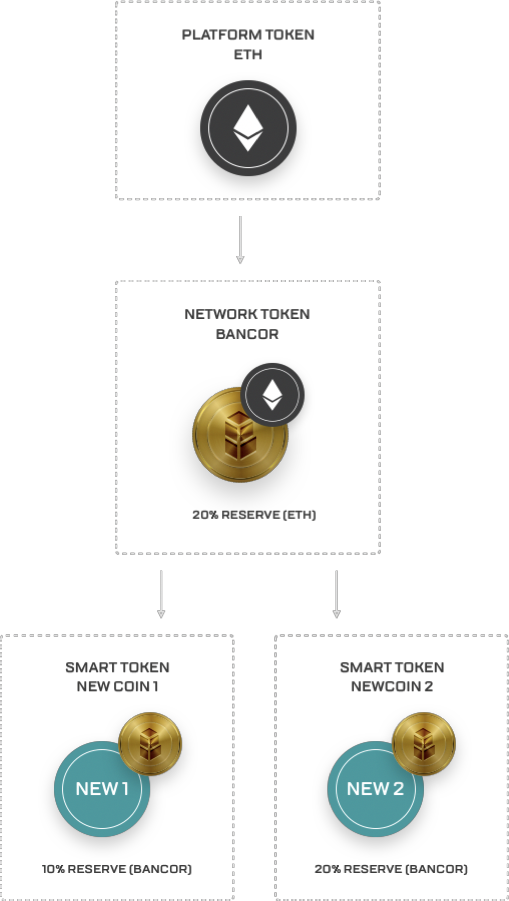
\includegraphics[keepaspectratio,scale=0.8]{fig1.png}
    \end{center}
   \end{wrapfigure} 
   \noindent

   300,000BNTが1対1の交換比率で発行され、クラウドセールの参加者に移される。240,000ETHはBNTプロジェクトが発展するための資金として差し向けられ、60,000ETH(CRRは20\%とする)はBNTのスマートコントラクト内に、準備残高として保持される。

   \begin{itemize}
    \item BNTを購入したり精算したりすることは、クラウドセールが完了すると同時に可能になる。取引開始時の価格は、クラウドセールにおける最後の価格になり、この例では、1ETHが最初のBNTの価格となる。
    \item BNTを精算する者は、BNTの準備残高のからETHを得る。精算されたBNTは破棄され、それにつれてBNTの価格が下がる。
    \item BNTを購入する者は、新たに作られたBNTを得る。ETHでの支払いはスマートコントラクトによる準備残高に追加され、BNTの価格は上がる。
   \end{itemize}

   ETHの準備残高は常に、BNTの時価総額の20\%のままであり続ける。

   \begin{figure}[h]
    \begin{center}
     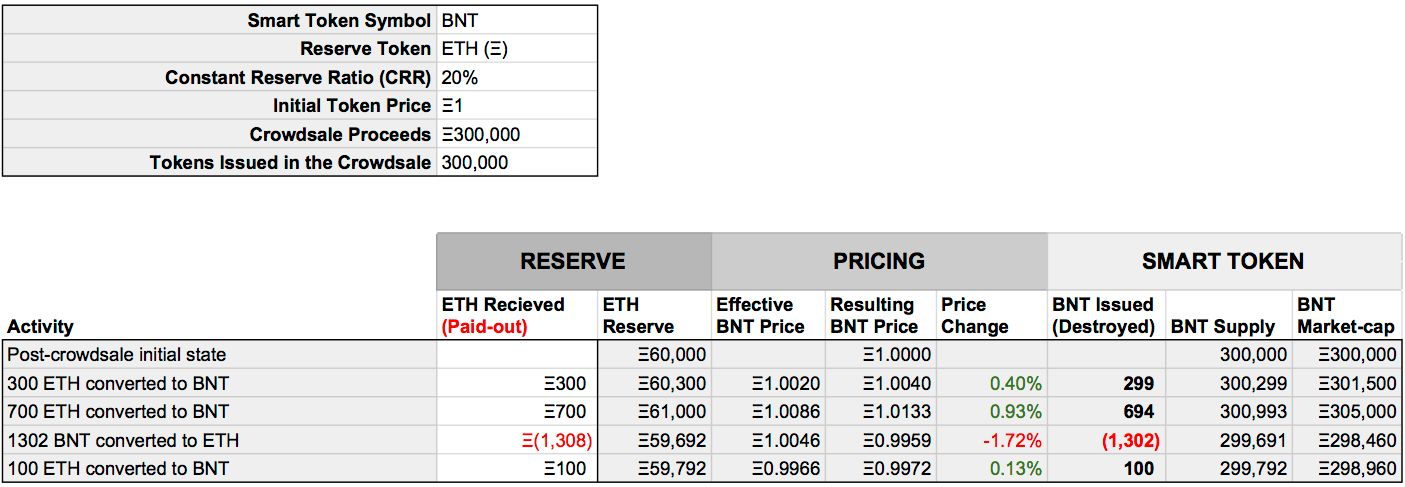
\includegraphics[scale=0.3]{fig2.png}
    \end{center}
   \end{figure}

   \href{https://goo.gl/3hR6e8}{スプレッドシートへのリンク}

  \subsection{例2:トークンチェンジャーの取引フロー}

  この例においては、BNTGNOという、BNTとGNO(Gnosis)のトークンチェンジャーとして機能するスマートトークンを扱う。BNTGNOは、BNTおよびGNOをそれぞれ50\%のCRRで準備トークンとして持ち、合わせて100\%のCRRとなる。

  \begin{wrapfigure}{r}{60mm}
    \begin{center}
     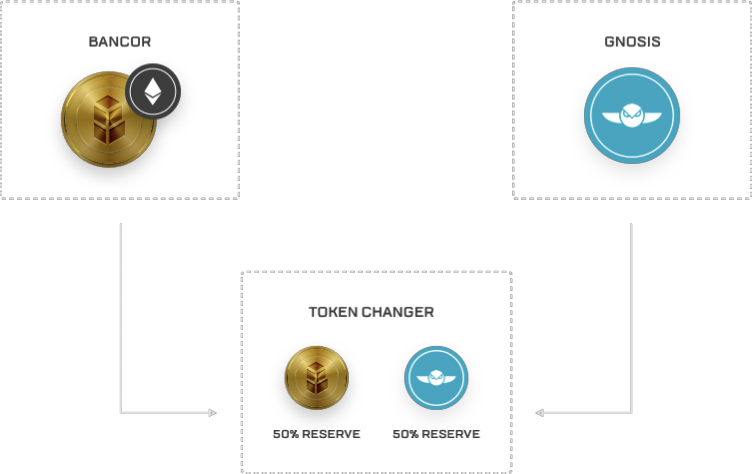
\includegraphics[keepaspectratio,scale=0.8]{fig3.png}
    \end{center}
   \end{wrapfigure} 
  \noindent

  現在の市場価格が$1 BNT = 2 GNO$という前提で、コントラクトにより初期価格が$1 BNT = 2 GNO = 1 BNTGNO$と定義されるとする。そして、この例では、10,000BNTGNOが発行され、最初の準備残高として預託される。

  \begin{itemize}
    \item 開始時の価格は$1 BNTGNO = 1 BNT = 2 GNO$としてコントラクトにコントラクト上に設定される。
    \item BNTGNOは、BNTでもGNOでも購入できる。BNTGNOの価格は、BNTあるいはGNOの、BNTGNOを購入した側に対して上昇し、(BNTGNOの供給量の増加により)、別の一方の準備トークンに対して下降する。
    \item BNTGNOは、BNTにもGNOにも精算できる。それにともない、精算された側の準備トークンに対してBNTGNOの価格は下降し、もう一方に対しては上昇する。
  \end{itemize}

  このシナリオは、50\%ずつのCRRを持つ準備トークンによって100\%の準備残高を持つスマートトークンが、誰に対しても開かれており、その価格が自然と裁定取引によってバランスするような、非中央集権的なトークンチェンジャーとして機能する実例を示すものである。トークンチェンジャーとトークンのバスケットが自動的にCRRの割合を維持することになる。

  \begin{figure}[h]
   \begin{center}
    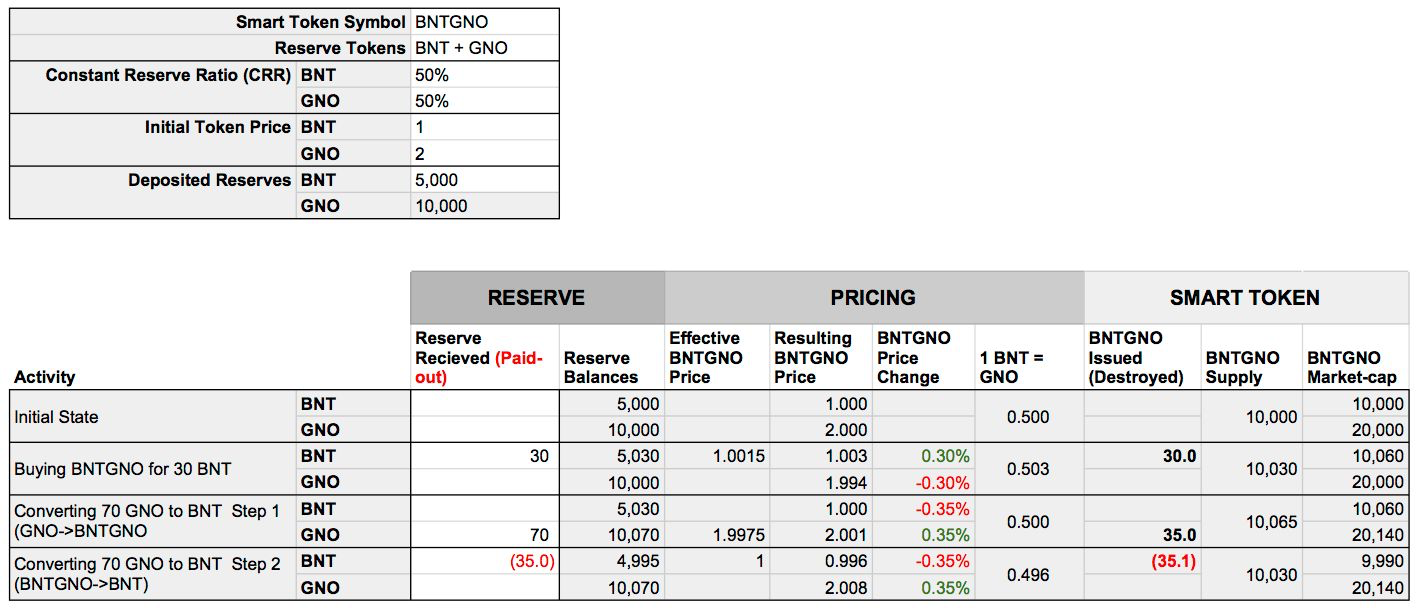
\includegraphics[scale=0.3]{fig4.png}
   \end{center}
  \end{figure}

  \href{https://goo.gl/3hR6e8}{スプレッドシートへのリンク}

  \subsection{潜在的なBancorネットワークの図解}

  下図において:

  \begin{itemize}
    \item BNTは、Etherにより実現するスマートトークンである。
    \item ETH、DGD、DGX、REP、GNTは、標準的なEthereumによるトークンである。
    \item NEWは、クラウドファンディングのキャンペーンや、コミュニティ通貨などによって新規に作成されるスマートトークンである。
    \item スマートトークンは、準備残高をもつ(矢印は、準備トークンを指し示す)。  
    \item トークンチェンジャーは、ふたつ以上の準備残高からなる100\%の準備残高に保証されている。
  \end{itemize}

  \begin{figure}[h]
   \begin{center}
    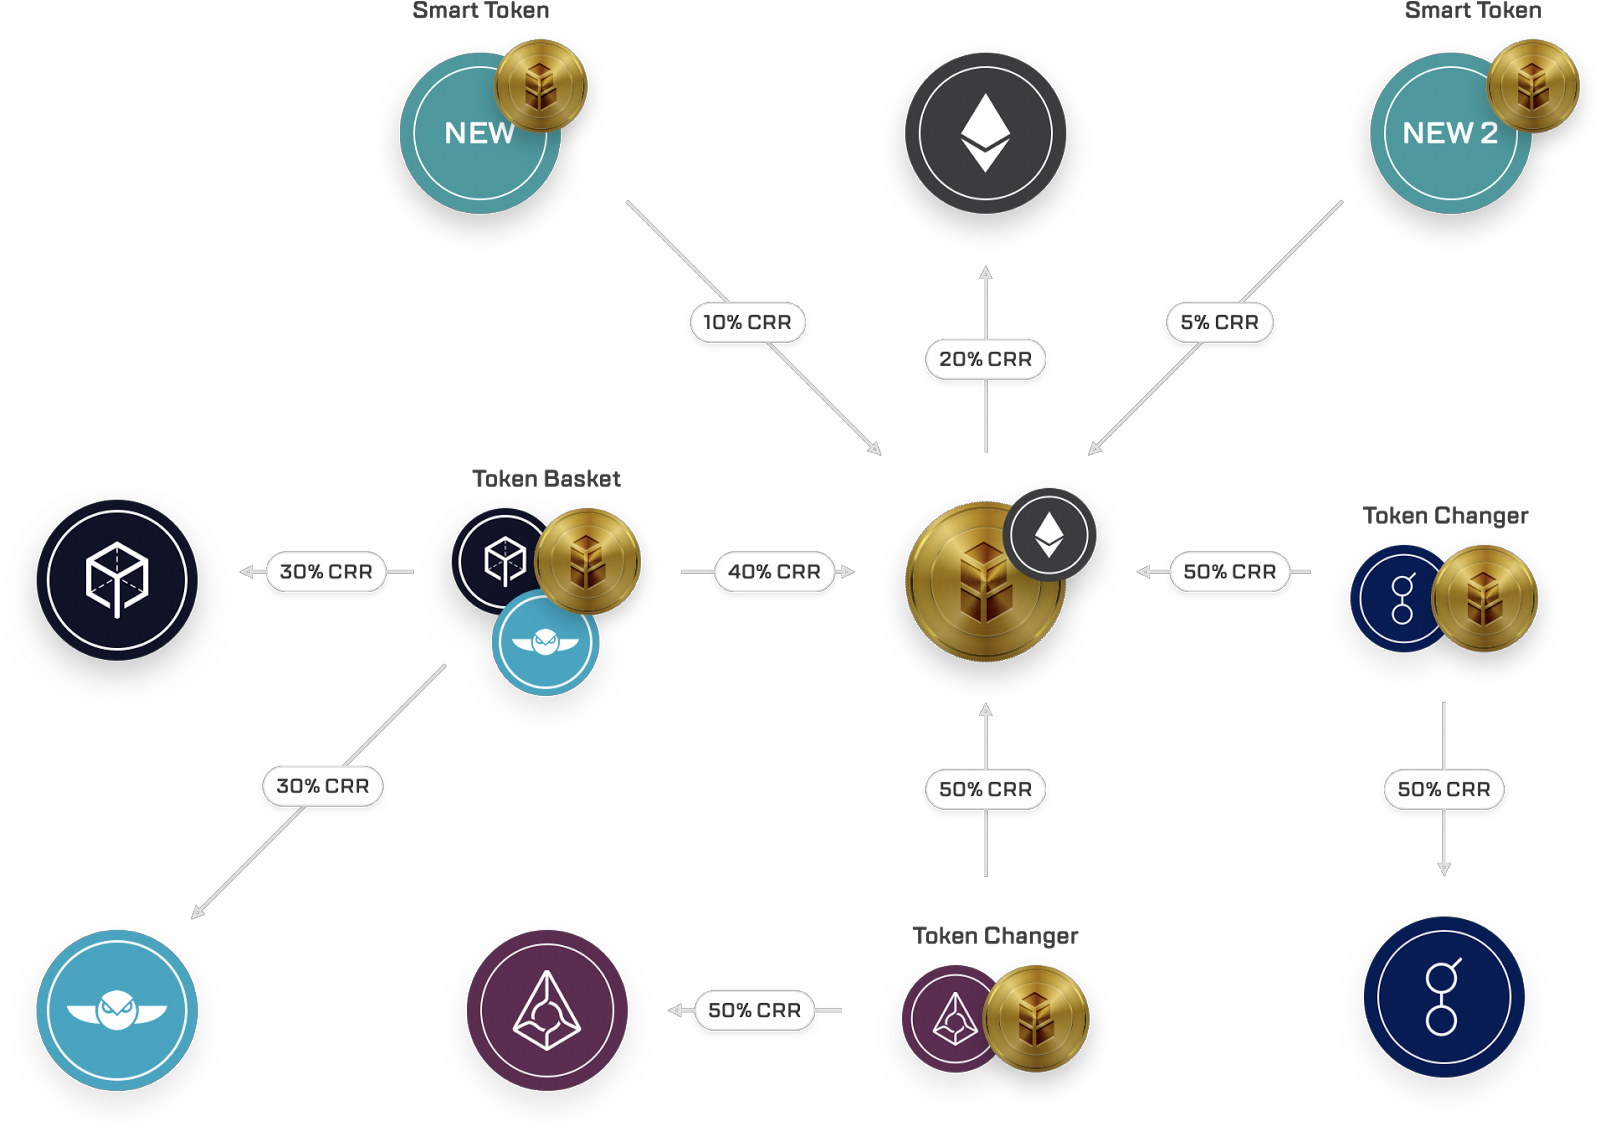
\includegraphics{fig5.png}
   \end{center}
  \end{figure}

\section{取引ごとの価格計算}

スマートトークンの価格計算は、実際には、トランザクションサイズの関数として計算される。

R:準備トークンの残高

S:スマートトークンの供給量

F:不変の準備率

\begin{itemize}
  \item $R$、$S$、$F$を上記の通りおく時、準備トークン$E$との交換において得られるスマートトークン$T$は
  \begin{equation*} \label{eq:price-discovery-formula}
    T = S((1 + \frac{E}{R})^F - 1)
  \end{equation*}

  \item $R$、$S$、$F$を上記の通りおく時、スマートトークン$T$との交換において得られる準備トークン$E$は
  \begin{equation*} \label{eq:price-discovery-formula}
    E = R(1 - F\sqrt{1 - \frac{T}{S}})
  \end{equation*}
\end{itemize}

\emph{\href{https://goo.gl/HXQBUr}{数学的証明}も用意している。}
\footnote{
  数学的証明は、\url{https://goo.gl/HXQBUr}にて、オンラインで閲覧できる。
}

\section{要約}

Bancorプロトコルは、スマートトークンを標準化し、スマートコントラクトを通じた不変の割合に基づく準備トークンの保有により、暗号通貨のための非同期的な価格発見と、継続的な流動性を可能にする。また、それは自動的な市場形成を実行する。Bancorプロトコルは、流動性リスクなしに、階層的な貨幣システムを作ることも可能にする。BNTスマートトークンは、最初の非中央集権的な、通貨交換システムを確立するために使われ、それは値付けのマッチングも注文の要求も行わないため、取引量と関係なく流動性を保つことができる。このシステムは、資産の交換における\emph{欲求の二重一致問題}に対する、初の技術的な解決策を提案する。そして、ユーザ作成通貨のロングテールの発生を可能にする。

\section{謝辞}

我々は、本文書を書くに際して支援してくれたたくさんの人々に感謝の意を表したい。Meni Rosenfeld、Yudi Levi、Amatzia Benartzi、Ron Gross、Assaf Bahat、Sefi Golan、Joshua Alliance、Brian Singerman、Adi Scope、Dory Asher、Tal Keinan、Wings.ai、TheFloor、Arie Ben-David(Israel Monetary Change Movement)、Scott Morris(Ithacash、そしてBancorチームのIlana、Asaf、Or、Omry、Itay、Matiには、特別の感謝の意を表する。読者諸賢が、もしこの文書の改善に対して支援やフィードバックをくださるなら、それはとても重要なことである。感謝申し上げる。

\end{document}
